
% Modelo de Trabalho Acadêmico da UNESP de Guaratinguetá v-2.0
% atualização Copyright 2024 by Biblioteca FEG UNESP com colaboração de Vitor Pinto Ribeiro and Gustavo Santos Borges and Ronaldo César de Paiva
% Modelo de Trabalho Acadêmico da UNESP de Guaratinguetá v-1.0
% original copyright 2017 by Eduardo Rohde Eras

% This program is free software: you can redistribute it and/or modify
% it under the terms of the GNU General Public License as published by
% the Free Software Foundation, either version 3 of the License, or
% (at your option) any later version.
%
% This program is distributed in the hope that it will be useful,
% but WITHOUT ANY WARRANTY; without even the implied warranty of
% MERCHANTABILITY or FITNESS FOR A PARTICULAR PURPOSE.  See the
% GNU General Public License for more details.
%
% You should have received a copy of the GNU General Public License
% along with this program.  If not, see <http://www.gnu.org/licenses/>.
%
%----------------------------------------------------------------------------------------%
%APRESENTAÇÃO 
% Este modelo pode ser usado como apoio para seu trabalho acadêmico e é destinado para ser usado no Word, não aplicável a outros editores de texto.
%
%Essas instruções são voltadas para a comunidade acadêmica da Universidade Estadual Paulista “Júlio de Mesquita Filho” (Unesp). Caso você seja de outra instituição, verifique as regras vigentes da sua universidade ou faculdade.
%
%O uso deste modelo não substitui o conhecimento das normas, diretrizes da universidade e orientações de seus professores e a Rede de Bibliotecas da Unesp está isenta de eventuais e quaisquer problemas ou prejuízos decorrentes do uso deste arquivo em softwares não licenciados, arquivos corrompidos, vírus ou quaisquer outros motivos.
%
%Em caso de dúvidas, consulte o Manual de normalização de trabalhos acadêmicos: apresentação: ABNT (2023): \url{https://docs.google.com/document/d/1ipkGiAUnAr_YBTrpFJpnud3aa4llBsROpBdkUfw91L0/edit?usp=sharing}
%----------------------------------------------------------------------------------------%
% C L A S S E   D O   D O C U M E N T O
%----------------------------------------------------------------------------------------%

\PassOptionsToPackage{colorlinks=true, allcolors=black}{hyperref}
\documentclass[
  %----------------------------------------------------------------------------------------%
  %Opções da classe 'memoir'
  %----------------------------------------------------------------------------------------%
  12pt,		% Tamanho da Fonte.
  a4paper,	% Tamanho da página.
  openright,  % Capítulos começam em páginas ímpares (insere uma página vazia se necessário).
  oneside,	% Para impressão em frente e verso utilizar twoside.
  %----------------------------------------------------------------------------------------%
  %Opções da classe 'abntex2'
  %----------------------------------------------------------------------------------------%
  chapter=TITLE,		%Títulos de capítulos convertidos em letras maiúsculas.
  section=TITLE,		%Títulos de seções convertidos em letras maiúsculas.
  %----------------------------------------------------------------------------------------%
  %Opções da classe 'babel'
  %----------------------------------------------------------------------------------------%
  english,	%Idioma adicional para hifenização.
  french,	    %Idioma adicional para hifenização.
  spanish,	%Idioma adicional para hifenização.
  brazil	    %Idioma principal do documento.
  %----------------------------------------------------------------------------------------%
]{abntex2}

%----------------------------------------------------------------------------------------%
% P A C O T E S
%
% Insira aqui os pacotes que for utilizar em seu documento. Para saber quais pacotes o
% template já está utilizando, confira o arquivo "pacoteBasico.sty".
%----------------------------------------------------------------------------------------%
    
    \usepackage{pacoteBasico}   %Pacote Básico de formatação no padrão da UNESP/FEG
    \usepackage{color}		    %Controle das cores.
    \usepackage{graphicx}	    %Inclusão de gráficos.
    \usepackage{lipsum}		    %Para geração de 'Dummy Text'.
    \usepackage{pdfpages}       %Para inclusão de arquivos pdf
    \usepackage[table,xcdraw]{xcolor}
    
%----------------------------------------------------------------------------------------%
% I N F O R M A Ç Õ E S   B Á S I C A S   S O B R E   O   T R A B A L H O
%
% Defina aqui as informações pertinentes ao trabalho.
%----------------------------------------------------------------------------------------%

    %----------------------------------------------------------------------------------------%
    % D A D O S   P E S S O A I S
    %----------------------------------------------------------------------------------------%
    
    %Nome completo do autor do presente Trabalho acadêmico:
    \newcommand{\nomeDoAutor}{
    Nome Completo do Autor
    }
    
    %Nome do curso:
    \newcommand{\nomeDoCurso}{Nome do Curso}
    
    %----------------------------------------------------------------------------------------%
    % D A D O S   S O B R E   O   T R A B A L H O
    %----------------------------------------------------------------------------------------%
    
    %Título do presente trabalho:
    \newcommand{\tituloDoTrabalho}{
    Título do trabalho acadêmico
    }
      
    %Subtítulo do presente trabalho, se houver:
    \newcommand{\subtituloDoTrabalho}{
    subtítulo se houver
    }
    
     %Tipo do trabalho (Dissertação / Tese / Trabalho de Conclusão de Curso / Trabalho de Conclusão de Residencia) 
    \newcommand{\tipoDeTrabalho}{Tipo de Trabalho Acadêmico}

    % Nome da Faculdade ou instituto
    \newcommand{\NomeDaFaculdade}{Nome da Faculdade}

    %Grau acadêmico (Mestre(a) / Doutor(a) / Bachareal / Licenciatura etc)
    \newcommand{\GrauAcademico}{Grau acadêmico}
   
    % área de concentração, se houver (muito utilizado no mestrado e doutorado) % remover no pacote básico se não houver 
    \newcommand{\AreaDeConcentracao}{
    Área de concentração
    }
    
    %Mês da entrega do trabalho 
    \newcommand{\dataDeDefesa}{
    99/99/9999
    }
    
    %Ano da entrega do trabalho
    \newcommand{\anoDeEntrega}{
    Ano
    }
    
    %----------------------------------------------------------------------------------------%
    % D A D O S   D O S   O R I E N T A D O R E S,   B A N C A   E   C O O R D E N A D O R
    %----------------------------------------------------------------------------------------%
    
    %Nome do orientador do presente trabalho:
    \newcommand{\nomeDoOrientador}{
    Nome Completo do Orientador
    }
    % acrescentar intituição 
    %Título do orientador:
    \newcommand{\tituloDoOrientador}{
    Profº Dr.
    }
    
    %Nome do coorientador, se houver:
    \newcommand{\NomeDoCoorientador}{
    Nome Completo do Coorientador
    }
    
    %Título do coorientador:
    \newcommand{\tituloDoCoorientador}{
    Profº Dr.
    }
    
    %instituição do orientador 
    \newcommand{\instituicaoorientador}{Nome da Instituição do orientador}     
    
    %instituição do coorientador 
    \newcommand{\instituicaocoorientador}{Nome da Instituição do coorientador}
   
    %Nome do Membro da Banca 1 :
    \newcommand{\nomeDoMembroA}{Nome Completo do Membro da Banca}
    
    %Título do Membro da Banca 1:
    \newcommand{\tituloDoMembroA}{Profº Dr.}
    %instituição do Membro da Banca 1 
    \newcommand{\instituicaomembroA}{Nome da Instituição do membro 1}
    
    %Nome do membro da Banca 2:
    \newcommand{\nomeDoMembroB}{Nome Completo do Membro banca}
    
    %Título do Membro da Banca 2:
    \newcommand{\tituloDoMembroB}{Profº Dr.}
    % Instituição do Membro 2
    \newcommand{\instituicaomembroB}{Nome da Instituição do membro 2}
    
    %ATENÇÃO! Geralmente Tese de Doutorado possui mais de 2 membros na banca, então é possível remover no pacote básico. 
     %Nome do membro da Banca 3:
    \newcommand{\nomeDoMembroC}{Nome Completo do Membro banca}
    
    %Título do Membro da Banca 3:
    \newcommand{\tituloDoMembroC}{Profº Dr.}
    % Instituição do Membro 3
    \newcommand{\instituicaomembroC}{Nome da Instituição do membro 3}
     %Nome do membro da Banca 4:
    \newcommand{\nomeDoMembroD}{Nome Completo do Membro banca}
    
    %Título do Membro da Banca 4:
    \newcommand{\tituloDoMembroD}{Profº Dr.}
    % Instituição do Membro 4
    \newcommand{\instituicaomembroD}{Nome da Instituição do membro 4}
    %----------------------------------------------------------------------------------------%
    % D A D O S   D A   I N S T I T U I Ç Ã O
    %----------------------------------------------------------------------------------------%

    %Nome da Cidade de defesa
    \newcommand{\nomeDaCidade}{Cidade}
    
    %Nome da Universidade Nome da Faculdade ou Instituto - Campus nome da Cidade

    \newcommand{\nomeDaUniversidade}{
    UNIVERSIDADE ESTADUAL PAULISTA -- UNESP\\
    \NomeDaFaculdade -- Campus de\ \nomeDaCidade
    }
    
    

%----------------------------------------------------------------------------------------%
% I N Í C I O   D O   D O C U M E N T O - P R É   T E X T U A L

%----------------------------------------------------------------------------------------%
\begin{document}
    
    \imprimircapa
    \imprimirfolhaderosto
    
    %------------------------------------------------------------------------------------%
    %ELEMENTO OPCIONAL. Consulte a seção de pós-graduação da sua unidade e verifique a obrigatoriedade ou não deste item. Se não ouver necessidade, exclua essa página. 
    
     \begin{resumo}[IMPACTO POTENCIAL DESTA PESQUISA]
O impacto esperado na sociedade deve ser redigido de forma sucinta considerando, os seguintes aspectos: o potencial científico, técnico, social, inovador, econômico, educacional e cultural; a internacionalização; a inserção local, regional e nacional;  o desenvolvimento sustentável, conhecimento e temática da pesquisa. 

\vspace*{0.5cm}
        
        %Subistitua pela palavra no idioma desejado, caso precise.
        \begin{center}
            \noindent\textbf{\MakeUppercase{POTENTIAL IMPACT OF THIS RESEARCH }}
        \end{center}
        

\vspace*{0.5cm}

The expected impact on society should be written succinctly, considering the following aspects: the scientific, technical, social, innovative, economic, educational and cultural potential; internationalization; local, regional and national insertion; sustainable development, knowledge and research themes.

      \end{resumo}
      
    % F O L H A   D E   A P R O V A Ç Ã O
    %
    % OBRIGATÓRIO. Este é o modelo de folha de aprovação que deve ser digitalizada após as assinaturas da banca. Utilize um software de edição de PDF para substituição posterior dessa folha. Se possível, utilize um recurso de assinatura digital fornecido pela ferramenta de edição de PDF, evitando assim a digitalização da folha toda.
    %------------------------------------------------------------------------------------%
    \begin{folhadeaprovacao}
            
        \begin{center}
        \normalsize{\textbf{\MakeUppercase\nomeDoAutor}}
        \\
        \vspace*{1cm}
        \normalsize{\textbf{\MakeUppercase\tituloDoTrabalho:}}
        \\
        \subtituloDoTrabalho
        \end{center}
                
        \vspace*{2cm}
        
            \noindent\tipoDeTrabalho\ apresentado(a) à Universidade Estadual Paulista (UNESP),\ \NomeDaFaculdade,\ \nomeDaCidade, para obtenção do título de\ \GrauAcademico{ }em\ \nomeDoCurso.
            \par
            \vspace*{1cm} 
         \noindent {Área de Concentração: \AreaDeConcentracao}
          
            \vspace*{1cm} 
       
       \noindent Data de defesa: \dataDeDefesa
        \vspace*{1cm}
       
       \noindent{BANCA EXAMINADORA}
       
       \vspace*{1cm}
       
       \raggedright\makebox[2.5in]{\hrulefill}\\
       \tituloDoOrientador \nomeDoOrientador \\ UNESP -- \NomeDaFaculdade\ -- Campus de \nomeDaCidade

       \vspace*{1cm}
       
       \raggedright\makebox[2.5in]{\hrulefill}\\
       \tituloDoMembroA\ \nomeDoMembroA \\ \instituicaomembroA

       \vspace*{1cm}
       
       \raggedright\makebox[2.5in]{\hrulefill}\\
       \tituloDoMembroB\ \nomeDoMembroB \par \instituicaomembroB
       
       \vspace*{1cm}
       
       \raggedright\makebox[2.5in]{\hrulefill}\\
       \tituloDoMembroC\ \nomeDoMembroC \\ \instituicaomembroC
       
       \vspace*{1cm}
       
       \raggedright\makebox[2.5in]{\hrulefill}\\
       \tituloDoMembroD\ \nomeDoMembroD \\ \instituicaomembroD
       
    \end{folhadeaprovacao}
    
   
    %------------------------------------------------------------------------------------%
    % D E D I C A T Ó R I A
    %
    % ELEMENTO OPCIONAL. Se não for utilizar uma dedicatória, basta apagar todo o código dessa seção.
    %------------------------------------------------------------------------------------%
    
    \begin{dedicatoria}
        \vspace*{\fill}
        \begin{flushright}
                       Dedico este trabalho à … 
        \end{flushright}
        \vspace*{1cm}
    \end{dedicatoria}

    %------------------------------------------------------------------------------------%
    % A G R A D E C I M E N T O S
    %
    % ELEMENTO OPCIONAL. PORÉM É OBRIGATÓRIO PARA BOLSISTAS. 
    % Citar as pessoas, instituição, agência de fomento, entre outros que contribuíram de maneira relevante à elaboração do trabalho e na vida acadêmica.
    % Se não for utilizar os agradecimentos, basta apagar todo o código dessa seção.
    %------------------------------------------------------------------------------------%
    \begin{agradecimentos}
                  
        É um texto em que o autor agradece as pessoas que contribuíram de forma relevante para o desenvolvimento do trabalho, quando houver apoio financeiro à pesquisa, deve-se obrigatoriamente mencionar esse apoio nos agradecimentos, conforme o que prevê cada agência.
        
        O presente trabalho foi realizado com apoio da Coordenação de Aperfeiçoamento de Pessoal de Nível Superior – Brasil (CAPES) – Código de Financiamento 001.
        
        À FAPESP, pelo apoio financeiro, concedido por meio do Processo nº aaaa/nnnnn-d, Fundação de Amparo à Pesquisa do Estado de São Paulo (FAPESP).
        
        Ao Conselho Nacional de Desenvolvimento Científico e Tecnológico (CNPq), pela concessão de bolsa de pesquisa (processo XXX).

    
    \end{agradecimentos}
    
    %------------------------------------------------------------------------------------%
   
    %------------------------------------------------------------------------------------%
    % E P Í G R A F E
    %
    % ELEMENTO OPCIONAL. Texto em que o autor apresenta uma citação, seguida de indicação de autoria.
    % Se não for utilizar uma epígrafe, basta apagar todo o código dessa seção.
    %------------------------------------------------------------------------------------%
    
    \begin{epigrafe}
        \vspace*{\fill}
    	\begin{flushright}
    		\textit{
        		``As universidades serão o que são suas bibliotecas``\\ 
        		\cite[~ p. 19, tradução nossa]{Gelfand}
            		}
    	\end{flushright}
    \end{epigrafe}
    
    %------------------------------------------------------------------------------------%
    % R E S U M O   N O   I D I O M A   D O   T E X T O
    %
    % OBRIGATÓRIO. Elaborado conforme a NBR 6028. 
    % Deve ser redigido em um só parágrafo contendo de 150 a 500 palavras e ressaltar: objetivo, método, resultados e as principais conclusões.
    % Após o resumo, são listadas palavras-chave relacionadas à temática do trabalho, separadas entre si por ponto e virgula (;) e finalizadas por ponto final.  (NBR 6028)
    %------------------------------------------------------------------------------------%
    
    \begin{resumo}
    
    O texto deve ser composto por frases concisas em parágrafo único, utilizando o verbo na terceira pessoa. Evite símbolos e contrações que não sejam de uso corrente. Evite fórmulas, equações, diagramas etc., que não sejam absolutamente necessários; quando seu emprego for imprescindível, defini-los na primeira vez que aparecerem. Um resumo deve conter entre 150 a 500 palavras. As palavras-chave devem ficar logo abaixo do resumo, separadas entre si por ponto e vírgula e finalizadas por ponto. Além disso, devem ser grafadas com as iniciais em letra minúscula, exceto nomes próprios e nomes científicos. Para a escolha das palavras-chave consulte o Tesauro Unesp ou descritores autorizados da área, que representam o conteúdo do trabalho.
        
        \vspace*{0.5cm}
    
        \noindent\textbf{{Palavras-Chave: }} palavra-chave; palavra-chave; palavra-chave.
    
    \end{resumo}
    
    %------------------------------------------------------------------------------------%
    % A B S T R A C T :   R E S U M O   N O   I D I O M A   E S T R A N G E I R O
    %
    % OBRIGATÓRIO. Elaborado com as mesmas características do resumo em língua portuguesa.
    % Se redigido em inglês-ABSTRACT, em castelhano-RESUMEN, em francês-RÉSUMÉ.
    % Após o resumo, são listadas palavras-chave relacionadas à temática do trabalho no 
    % idioma escolhido. Se redigido em inglês - KEYWORDS, em espanhol - PALABRAS CLAVES,
    % em francês - MOTS-CLÉS.
    % TEXTO ATUAL 
    %ZUSAMMENFASSUNG (alemão)
    %RIASSUNTO (italiano)

    %Keywords (inglês)
    %Palabras clave (espanhol)
    %Mot-clé (francês)
    %Stichwörter (alemão)
    %Parole chiave (italiano)
    %------------------------------------------------------------------------------------%
    
    \begin{resumo}[Abstract] % Substitua 'Abstract' pela palavra no idioma desejado, caso precise.
    
    The text should consist of concise sentences in a single paragraph, using the third person singular form of the verb. Avoid symbols and contractions that are not commonly used. Avoid formulas, equations, diagrams, etc., unless absolutely necessary; when their use is essential, define them the first time they appear. An abstract should contain between 150 to 500 words. Keywords should be placed right below the abstract, separated by semicolons and ending with a period. Additionally, they should be written in lowercase except for proper names and scientific names. To choose keywords, consult the Tesauro Unesp or authorized descriptors in the field that represent the content of the work.
        
        \vspace*{0.5cm}
        
        %Subistitua 'Keywords' pela palavra no idioma desejado, caso precise.
        \noindent\textbf{{Keywords: }} keyword; keyword; keyword.
    
    \end{resumo}
    
    %------------------------------------------------------------------------------------%
    % L I S T A   D E   I L U S T R A Ç Õ E S
    %
    % ELEMENTO OPCIONAL. Deve ser elaborada de acordo com a ordem em que se apresenta no texto, podendo ser em lista própria para cada tipo de ilustração ou lista única para variados tipos de ilustrações (figuras, fotografias, organogramas, quadros, etc).(NBR: 14724)
    % Se não for utilizar uma Lista de Ilustrações, basta apagar todo o código dessa seção.
     
    
    %------------------------------------------------------------------------------------%
    
    \listoffigures*
    \newpage
    
    %------------------------------------------------------------------------------------%
    % L I S T A   D E   T A B E L A S
    %
    % ELEMENTO OPCIONAL. Deve ser elaborada de acordo com a ordem em que se apresenta no texto.
    %Se não for utilizar uma Lista de Tabelas, basta apagar todo o código dessa seção.
    %------------------------------------------------------------------------------------%
    
    \listoftables*
    \newpage
    
    %------------------------------------------------------------------------------------%
    % L I S T A   D E   A B R E V I A T U R A S   E   S I G L A S
    %
    % ELEMENTO OPCIONAL. Deve ser elaborada em ordem alfabética, seguidas das palavras ou expressões correspondentes por extenso.
    % Se não for utilizar uma Lista de Abreviaturas, basta apagar todo o código dessa seção.
   
    %------------------------------------------------------------------------------------%
    
    \begin{siglas}
        \item [ACT]	Administração Científica do Trabalho 
        \item [AIT]	Associação Internacional do Trabalho 
        \item [CAPES]	Coordenação de Aperfeiçoamento de Pessoal de Nível Superior 
        \item [IES]	Instituição de Ensino Superior 
        \item [MEC]	Ministério da Educação 
        \item [OMS]	Organização Mundial da Saúde
    \end{siglas}  

    
    %------------------------------------------------------------------------------------%
    % L I S T A   D E   S Í M B O L O S
    %
    % ELEMENTO OPCIONAL. Deve ser elaborada de acordo com a ordem em que se apresenta no texto, acompanhado com seus respectivos significados. Se não for utilizar uma Lista de Símbolos, basta apagar todo o código dessa seção.
    
    %------------------------------------------------------------------------------------%
    
    \begin{simbolos}
        \item[$\alpha$] Letra Grega Alfa
        \item[$\beta$] Letra grega Beta
        \item[$\gamma$] Letra grega Gama
        \item[$e$] Número de Euler
        \item[R\$] Unidade monetária Brasileira (Real)
    \end{simbolos}
    
    %------------------------------------------------------------------------------------%
    % S U M Á R I O
    %
    % OBRIGATÓRIO. Recomenda-se atualizar o sumário apenas no fim da elaboração do trabalho. 
    % Havendo mais de um volume, cada um deve conter o sumário completo do trabalho (NBR: 6024; NBR: 6027). 
    % Não se deve confundir sumário com índice.
    
    %------------------------------------------------------------------------------------%
    
    \tableofcontents*
    \newpage
    
    %------------------------------------------------------------------------------------%
    %                                                                                    %
    %                           C O R P O   D O   T E X T O                              %
    %                                                                                    %
    %                     Seu trabalho começa a ser digitado aqui.                       %
    %                                                                                    %
    % Início do corpo do texto. A partir desse comando será impresso o número de páginas.% 
    %------------------------------------------------------------------------------------%
    
    \textual
    \pagestyle{simple} 
    
    %------------------------------------------------------------------------------------%
    
    \chapter{Introdução} % ELEMENTO OBRIGATÓRIO
    
    A introdução é a parte inicial do trabalho que apresenta o objetivo da pesquisa, a justificativa e sua importância para a área, a problemática e suas limitações. Deve ser redigido de forma sucinta, clara e objetiva. 
    %Em caso de dúvidas, consulte o Manual de normalização de trabalhos acadêmicos: apresentação: ABNT (2023): \url{https://docs.google.com/document/d/1ipkGiAUnAr_YBTrpFJpnud3aa4llBsROpBdkUfw91L0/edit?usp=sharing}
       
    
    \chapter{DESENVOLVIMENTO} % Elemento obrigatório
    
        
        O desenvolvimento do texto é a parte principal do trabalho, onde o tema será amplamente desenvolvido e apresentado. A exposição do assunto deve ser ordenada e pormenorizada, dividida em seções e subseções, que vão variar em função da abordagem do tema e da metodologia adotada. Em geral, é composto pelos seguintes tópicos/divisões: Proposição; Revisão da literatura; Material e Método; Resultado e Discussão. Recomenda-se consultar seu/sua orientador/a para definir o formato e apresentação do texto no desenvolvimento do seu trabalho.
                
        
           
    \chapter{REGRAS DE APRESENTAÇÃO} 
    % % Nesse capítulo será ilustrado como se utilizar os diferentes níveis e subníveis de seção em seu documento. 
    %Fique atento quanto a identação do código para manter a clareza e organização de seu trabalho.
    % ATENÇÃO para todo título de segunda seção (nivel 2) deve ser escrita OBRIGATORIAMENTE com letras maiúsculas. Esse padrão deve ser mantido em todo texto que irá ajudar no sumário.

        Esse capítulo traz vários exemplos para a redação do trabalho acadêmico confome a NBR 14724 \cite{NBR14724}. Após a leitura, apague seu conteúdo ou reutilize as seções para a elaboração do seu trabalho acadêmico.

    \section{ALÍNEAS E SUBALÍNEAS} 

        De acordo com Norma Brasileira 6024, da Associação Brasileira de Normas Técnica \cite{NBR6024}, caso seja necessário elencar assuntos que não possuam títulos dentro de uma mesma seção, estes podem ser subdivididos em alíneas e subalíneas:
        
    \begin{enumerate}[label=\alph*)]
        \item exemplo de uma alínea: o texto que vem dentro da alínea é separado por ponto e vírgula;
        \item exemplo de uma segunda alínea: o texto que finaliza a alínea termina em ponto final:
        \begin{itemize}
            \item[--] exemplo de subalínea.
        \end{itemize}
    \end{enumerate}       

     \section{CITAÇÕES}

        Esse capítulo apresenta regras e exemplos para a elaboração de citações. As citações devem ser apresentadas conforme a NBR 10520 \cite{NBR10520}, e devem ser usadas em conjunto com a norma de referências, a \citeonline{NBR6023}.
        Nesta seção serão apresentados alguns exemplos de citações mais utilizadas. Para os demais tipos, consulte o e-book: Manual de normalização de trabalhos acadêmicos: citação e referência: ABNT \cite{unesp2020ref}.
      

    \subsection{Citações diretas}

        Citação direta é a transcrição textual de parte da obra do autor consultado. A indicação de paginação ou localização é obrigatória.
        
    \subsubsection{Citação direta com menos de quatro linhas}

        Indicar o trecho com aspas duplas. Exemplo:
        Segundo \citeonline[~ p.276]{Rouanet}, “[...] não somos humanos fora da cultura, mas não seremos homens livres se não pudermos, sempre que necessário, assumir uma posição de exterioridade com relação ao mundo social”.

    \subsubsubsection{Citação direta com quatro ou mais linhas}	

        Indicar com fonte tamanho 10, espaçamento simples e sem aspas. Recomenda-se o recuo de 4 cm da margem esquerda. Exemplo:
         % Utilize esse código toda a vez que for fazer uma citação direta com mais de 3 linhas. Mantenha todos os valores de alinhamento conforme o exemplo, substitua somente o conteúdo do texto pelo texto que irá utilizar.
         \vspace{1.5pt}
            \begin{flushright}
                \begin{minipage}{.724\textwidth}
                    {\SingleSpacing\small

                    Mas não há ninguém tão assustado, ou que tenha medos tão estranhos, quanto os conquistadores. Eles evocam intermináveis fantasmas, aterrorizados com a ideia de que suas vítimas um dia façam com eles o que fizeram com elas... mesmo que, na verdade, as vítimas não deem a mínima para essa mesquinharia e tenham seguido em frente \cite[~ p.253]{Jemisin}
                    }
                \end{minipage}
            \end{flushright}
            \vspace{1.5pt}
        
     
   \subsection{Citações indiretas}	

        Citação indireta é o texto baseado na obra do autor consultado. A indicação da página ou localização é opcional. Exemplo:
        
        Segundo Daniel Munduruku \cite{aruju}, cabe aos adultos oferecer condições às crianças para que elas se desenvolvam plenamente para que possam se tornar humanos completos. Assim, segundo o educador, é preciso educar as crianças para o agora, para o presente, sem pular as etapas da vida, pois pensar o futuro é renunciar o presente.

    \subsection{Citação de citação}	

        Define-se como texto citado por outro autor dentro do documento que está sendo consultado, do qual não se teve acesso ao original. Exemplo:
        \\
        Segundo Freire (1994, p. 13, \textit{apud} \cite[p.17]{streck}, “[...] a pedagogia do oprimido como centro, me aparecem tão atuais quanto outros a que me refiro dos anos 80 e de hoje”.
      
        % Para citação de citação descreva o sobrenome do autor da obra que não teve acesso,´entre parenteses indique o ano e página se houver e acrescente a expressão apud e a citação do autor que tem acesso inclusive a página) 
    
    
    \section{EQUAÇÕES E FÓRMULAS}
        
        Devem ser destacadas no texto de modo a facilitar sua leitura, se necessário, numeradas sequencialmente com algarismos arábicos entre parênteses, alinhado à direita. 
          \begin{equation}
            \label{eq:integral}
            \int\limits_a^b f(x) dx = \lim_{x \to \infty} \displaystyle\sum_{i=1}^{n} f(x_i) \Delta i
        \end{equation}        
     
      ORIENTAÇÃO: toda expressão que se deseja destacar do texto deve ser redigida dentro do ambiente \verb|equation| que oferece uma melhor compatibilidade, maior flexibilidade além de referências cruzadas. A equação \ref{eq:integral}  
        
    ATENÇÃO: Uma expressão matemática simples pode ser incluída no corpo do texto para elaboração de um raciocínio utilizando  ambiente matemático indicado pelos símbolos "\$\$", por exemplo,  o triângulo $a^2 = b^2 + c^2$ . Porém,  ambiente matemático indicado pelos símbolos "\$\$" deve ser EVITADO para qualquer expressão matemática que precisa ser destacada.
                  
        
    \section{ILUSTRAÇÕES}
        
         São consideradas ilustrações: desenhos, esquemas, fluxogramas, fotografias, gráficos, mapas, organogramas, plantas, quadros, retratos, figuras, imagens, entre outros. Veja exemplo \ref{figura:ex}:
         % Para que a ilustração fique próxima ao texto a que se refere, para isso, dentro do ambiente figure, inclua o comando \label{nome da figura} e no texto indique \ref e selecione o nome da figura. 
         % ORIENTAÇÃO: já foi pré definido em \latex  Parte superior: 
            % Formatação: fonte tamanho 12, espaçamento 1,5
            % Parte inferior: 
            % Formatação: fonte tamanho 10, espaçamento simples.  Atenção, não esquecer de incluir a fonte consultada, mesmo que tenha sido elaborada pelo autor do trabalho            
                \begin{figure}[h]
                    \centering
                    \caption{Banner da Semana do Livro e das Bibliotecas da Unesp 2022: Centenário da Semana de Arte Moderna }
                    
\includegraphics[width=1.0\linewidth,scale=1.0]{banner semana.png}
                    \par
                    {\small Fonte: \citeonline{banner}}
                    \par
                    {\small Legenda: Fundo bege com logo em cinza e vermelho. Com escritos em cinza: Semana do Livro e das Bibliotecas da Unesp, escrito em vermelho: 2022 Centenário da semana de arte moderna. }
                    \label{figura:ex}
                \end{figure}
    
    ATENÇÃO: Existem muitas formas diferentes de formatar um elemento utilizando os recursos do \LaTeX, o importante é manter a descrição, a referência e a formatação do elemento gráfico conforme o padrão. Observe o exemplo no \ref{quadro:ex}.
                       
                                
                \begin{itemize}
                    \item os quatro lados fechados;
                    \item traços horizontais e verticais;
                    \item identificação (Título) localizada na parte superior.
                \end{itemize}
                
               ORIENTAÇÃO: usar o  ambiente \verb|quadro| que foi especialmente criado para esse template, definido no arquivo \verb|pacoteBasico.sty|. Dentro desse ambiente é criado uma tabela (ambiente \verb|tabular|). Por padrão, todos os quadros serão listados na lista de figuras.
                % Para que o quadro fique próxima ao texto a que se refere, para isso, dentro do ambiente quadro, inclua o comando \label{nome do quadro} e no texto indique \ref e selecione o nome do quadro. 
        \begin{quadro}[H]
        \centering
        \caption{Atribuição do título das seções.}
            \begin{tabularx}{\columnwidth}{|X|X|X|X|X|}
            \hline
            Indic. numérico & Título da seção & Indicativo da seção & Sugestão do destaque tipográfico & Comando \\ \hline
            
            \textbf{1} & \textbf{INTRODUÇÃO} & \textbf{seção primária} & \textbf{LETRAS MAIÚSCULAS EM NEGRITO} & \textit{\textbackslash chapter}\{\} \\ \hline

            \textbf{2} & \textbf{A CRIAÇÃO ARTÍSTICA} & \textbf{seção primária} & \textbf{LETRAS MAIÚSCULAS EM NEGRITO} & \textit{\textbackslash chapter}\{\} \\ \hline

            2.1 & O PROCESSO DE CRIAÇÃO & seção secundária & LETRAS MAIÚSCULAS E SEM NEGRITO  & \textit{\textbackslash section}\{\} \\ \hline %(excepcionalmente para essa seção, deve  digitar o título em caixa alta (MAIÚSCULO)

            2.1.1 & Da intenção à realização & seção terciária & Primeira letra da   primeira palavra em maiúsculo e sem negrito & \textit{\textbackslash subsection}\{\} \\ \hline

            \textit{\textbf{2.1.1.1}} & \textit{\textbf{O artista como primeiro leitor de sua obra}} & \textit{\textbf{seção quaternária}} & \textit{\textbf{Primeira letra da primeira palavra em maiúscula, com negrito e itálico}} & \textit{\textbackslash subsubsection}\{\} \\ \hline

            \textit{2.1.1.2.1} & \textit{O espectador-artista} & \textit{seção quinária} & \textit{Primeira letra da primeira palavra em maiúscula e itálico} & \textit{\textbackslash subsubsubsection} \{\} \\ \hline

            \textbf{3} & \textbf{CONCLUSÃO} & \textbf{seção primária} & \textbf{LETRAS MAIÚSCULAS EM NEGRITO} & \textit{\textbackslash chapter}\{\} \\ \hline

            & \textbf{REFERÊNCIAS} & \textbf{seção primária} & \textbf{LETRAS MAIÚSCULAS EM NEGRITO, TÍTULOS SEM INDICATIVO NUMÉRICO} & \textbf{Consultar \textit{template}} \\ \hline

            & \textbf{APÊNDICES} & \textbf{seção primária} & \textbf{LETRAS MAIÚSCULAS EM NEGRITO} & \textbf{Consultar \textit{template}} \\ \hline

            & \textbf{ANEXOS} & \textbf{seção primária} & \textbf{LETRAS MAIÚSCULAS EM NEGRITO} & \textbf{Consultar \textit{template}}\\ \hline
            
        \end{tabularx} \label{quadro:ex}
        {\small Fonte: \citeonline{unesp2023for}}
        \end{quadro}
                                                         
                                 
             
    \section {Tabelas}
                 As tabelas trazem informações não discursivas com dados numéricos tratados estatisticamente e são padronizadas conforme as Normas de Apresentação Tabular do \citeonline{IBGE1993}. Deve ser citada no texto, inserida o mais próximo possível do trecho a que se referem. Observe o exemplo na Tabela \ref{tab:ex}.
                   % Para que a tabela fique próxima ao texto a que se refere, para isso, dentro do ambiente table, inclua o comando \label{nome da tabela} e no texto indique \ref e selecione o nome da tabela. 
                \begin{itemize}
                    \item lados esquerdo e direito da tabela sempre abertos;
                    \item partes superior e inferior sempre fechadas;
                    \item não há traços horizontais e verticais para separar números, em seu interior.
                \end{itemize}
                
                Observação: Devem conter a fonte mesmo que elaborada pelo autor.
                
                \begin{table}[H]
                    \centering
                    \caption{Trilhos fixos.}
                    \begin{tabular}{c|c|c|c|c|c}
                    \hline
                    Tipo & Trilho base [B] & Gabarito (ideal) [G] & Calço de enchimento [tc] & Presilha [tp] & Parafuso \\
                    \hline 
                    TR-37 & 122,2 & 194 & 7,9 & 9,5 & 22,2 \\
                    TR-45 & 130,2 & 202 & 9,5 & 9,5 & 22,2 \\
                    TR-50 & 136,5 & 208 & 9,5 & 12,5 & 25,4 \\
                    TR-52 & 131,7 & 204 & 9,5 & 12,5 & 25,4 \\
                    TR-57 & 139,7 & 212 & 9,5 & 12,5 & 25,4 \\
                    \hline
                    \end{tabular}
                    {\small Fonte: Elaborada pelos autores.}
                    \label{tab:ex}
                \end{table}

    \chapter{Conclusão}
                  
        Denominado também de considerações finais, é a parte final do texto, onde são apresentadas conclusões correspondentes aos objetivos ou hipóteses. É um processo de síntese dos principais resultados, com comentários do autor e as contribuições trazidas pelo trabalho. 
   
    %------------------------------------------------------------------------------------%
    %                               P Ó S   T E X T U A L                                %
    %                                                                                    %
    % Fim do corpo do texto. A partir desse comando as indicações no sumário serão       %
    % marcadas como 'pós textuais'.                                                      %
    %------------------------------------------------------------------------------------%
    
    \postextual
    
    %------------------------------------------------------------------------------------%
    % R E F E R Ê N C I A S
    %
    % OBRIGATÓRIO. Será gerada automaticamente a partir do arquivo "references.bib".
    %------------------------------------------------------------------------------------%
    
    \bibliography{references}

    
    
    %--------------------------------------------------------------------------------- 
    %GLOSSÁRIO 
    %
    % ELEMENTO OPCIONAL. É uma lista de termos, palavras ou expressões técnicas utilizadas no texto e acompanhadas de seus respectivos significados, ordenada alfabeticamente. deve iniciar em página distinta, logo após a bibliografia consultada, se houver; deve conter o título GLOSSÁRIO, centralizado, em letras maiúsculas, e sem indicativo numérico.
    
    %usar esses comandos para incluir o glossário e que apareça no sumário: \clearpage   %\chapter*{GLOSSÁRIO} \addcontentsline{toc}{chapter}{GLOSSÁRIO} 
    %Se não for utilizar um Glossário , basta apagar todo o código dessa seção.
    %-----------------------
   
    \clearpage
    \chapter*{GLOSSÁRIO} \addcontentsline{toc}{chapter}{GLOSSÁRIO} 
    
    \noindent\textbf{Acervo:} conjunto de bens que integram o patrimônio de um indivíduo, de uma instituição, de uma nação, agrupados por atribuição de valor, segundo sua natureza cultural e seguindo uma lógica de organização.\\ \\
\textbf{Acessibilidade:} facilidade no acesso ao conteúdo e ao significado de um objeto digital.\\ \\
\textbf{Acesso aberto:}  refere-se à disponibilidade e acesso gratuito por qualquer pessoa aos resultados de pesquisas científicas. Baseia-se na premissa de que o conhecimento científico é um bem público e, portanto, deve estar disponível a todos.\\ \\
\textbf {Direito autoral ou direito de autor}: é um conjunto de privilégios conferidos por lei à pessoa física ou jurídica criadora da obra intelectual, para que ela possa usufruir de quaisquer benefícios morais e patrimoniais resultantes da exploração de suas criações.\\ \\
\textbf {Formato de arquivo:} atributo de um arquivo que descreve sua codificação e identificado pela extensão no final do nome do arquivo. Por exemplo: *.DOC, *.PDF, *.JPEG.\\ \\
\textbf {Metadados:} Dados estruturados que descrevem e permitem encontrar, gerenciar, compreender e/ou preservar documentos ao longo do tempo.\\ \\
\textbf {Repositório Institucional:} sistema de informação que visa armazenar, preservar, organizar, disseminar e promover acesso aberto à produção intelectual produzida nas instituições de ensino e pesquisa.\\ \\
\textbf {Submissão:} é o ato de entregar um documento técnico-científico no RI e/ou BD.
    

   %
    % A P Ê N D I C E S
    %
    % ELEMENTO OPCIONAL. Consiste em um texto ou documento elaborado pelo autor a fim de complementar
    % sua argumentação. Se necessário ter mais de um apêndice, basta adicionar cada um dentro de um dentro de um comando "\chapter". % Se não for utilizar um Apêndice, basta apagar
    % todo o código dessa seção.
    %------------------------------------------------------------------------------------%

    \begin{apendicesenv}
        
        \chapter{RESUMO DAS REGRAS DE ELABORAÇÃO DO TRABALHO ACADÊMICO }
\begin{table}[htb!]
\centering
\begin{tabular}{l|
>{\columncolor[HTML]{D3DFEE}}l }
\hline
\textbf{Configuração da página} & \begin{tabular}[c]{@{}l@{}}formato A4 (21 cm x 29,7 cm)\\ margens: \\    esquerda e superior: 3 cm\\    direita e inferior: 2 cm\end{tabular}                                                                                                                                                          \\ \hline
\textbf{Fonte}                  & \cellcolor[HTML]{A7C0DE}\begin{tabular}[c]{@{}l@{}}recomenda-se Arial ou Times New Roman ou similares \\ no caso de software livre, em cor preta\end{tabular}                                                                                                                                          \\ \hline
\textbf{Tamanho da fonte}       & \begin{tabular}[c]{@{}l@{}}texto geral: 12\\ citações, notas de rodapé, paginação, legendas e fontes \\ das ilustrações e das tabelas: 10\end{tabular}                                                                                                                                                 \\ \hline
\textbf{Espaçamento}            & \cellcolor[HTML]{A7C0DE}\begin{tabular}[c]{@{}l@{}}texto geral: espaçamento 1,5\\ citações com mais de três linhas, notas de rodapé, ficha \\ catalográfica, natureza, resumo e palavras-chave, legendas \\ e fontes das ilustrações e das tabelas, e referências: \\ espaçamento simples\end{tabular} \\ \hline
\textbf{Paginação}              & \begin{tabular}[c]{@{}l@{}}contagem: as páginas antes da introdução devem ser \\ contadas sequencialmente, exceto capa e ficha \\ catalográfica, mas não numeradas. \\ numeração: canto superior direito a partir da Introdução, \\ fonte tamanho 10\end{tabular}                                      \\ \hline
\textbf{Cada artigo}            & \cellcolor[HTML]{A7C0DE}\textbf{Verifique a norma da revista ou NBR 6022}                                                                                                                                                                                                                              \\ \hline
\end{tabular}
\end{table}
                  
    \end{apendicesenv}
    
    %------------------------------------------------------------------------------------%
    % A N E X O S
    %
    % OPCIONAL. Consiste em um texto ou documento não elaborado pelo autor que serve de
    % fundamentação, comprovação ou ilustração ao trabalho. Se necessário ter mais de um
    % anexo, basta adicionar cada um dentro de um dentro de um comando "\chapter".
    % Se não for utilizar nenhum Anexo, basta apagar todo o código dessa seção.
    %------------------------------------------------------------------------------------%
    
    \begin{anexosenv}
    
        \chapter{PADRÃO DE FILIAÇÃO PARA TODAS AS PUBLICAÇÕES CIENTÍFICAS DA UNIVERSIDADE}
        %Utilizar o comando \includepdf para incluir arquivos no formato pdf.
            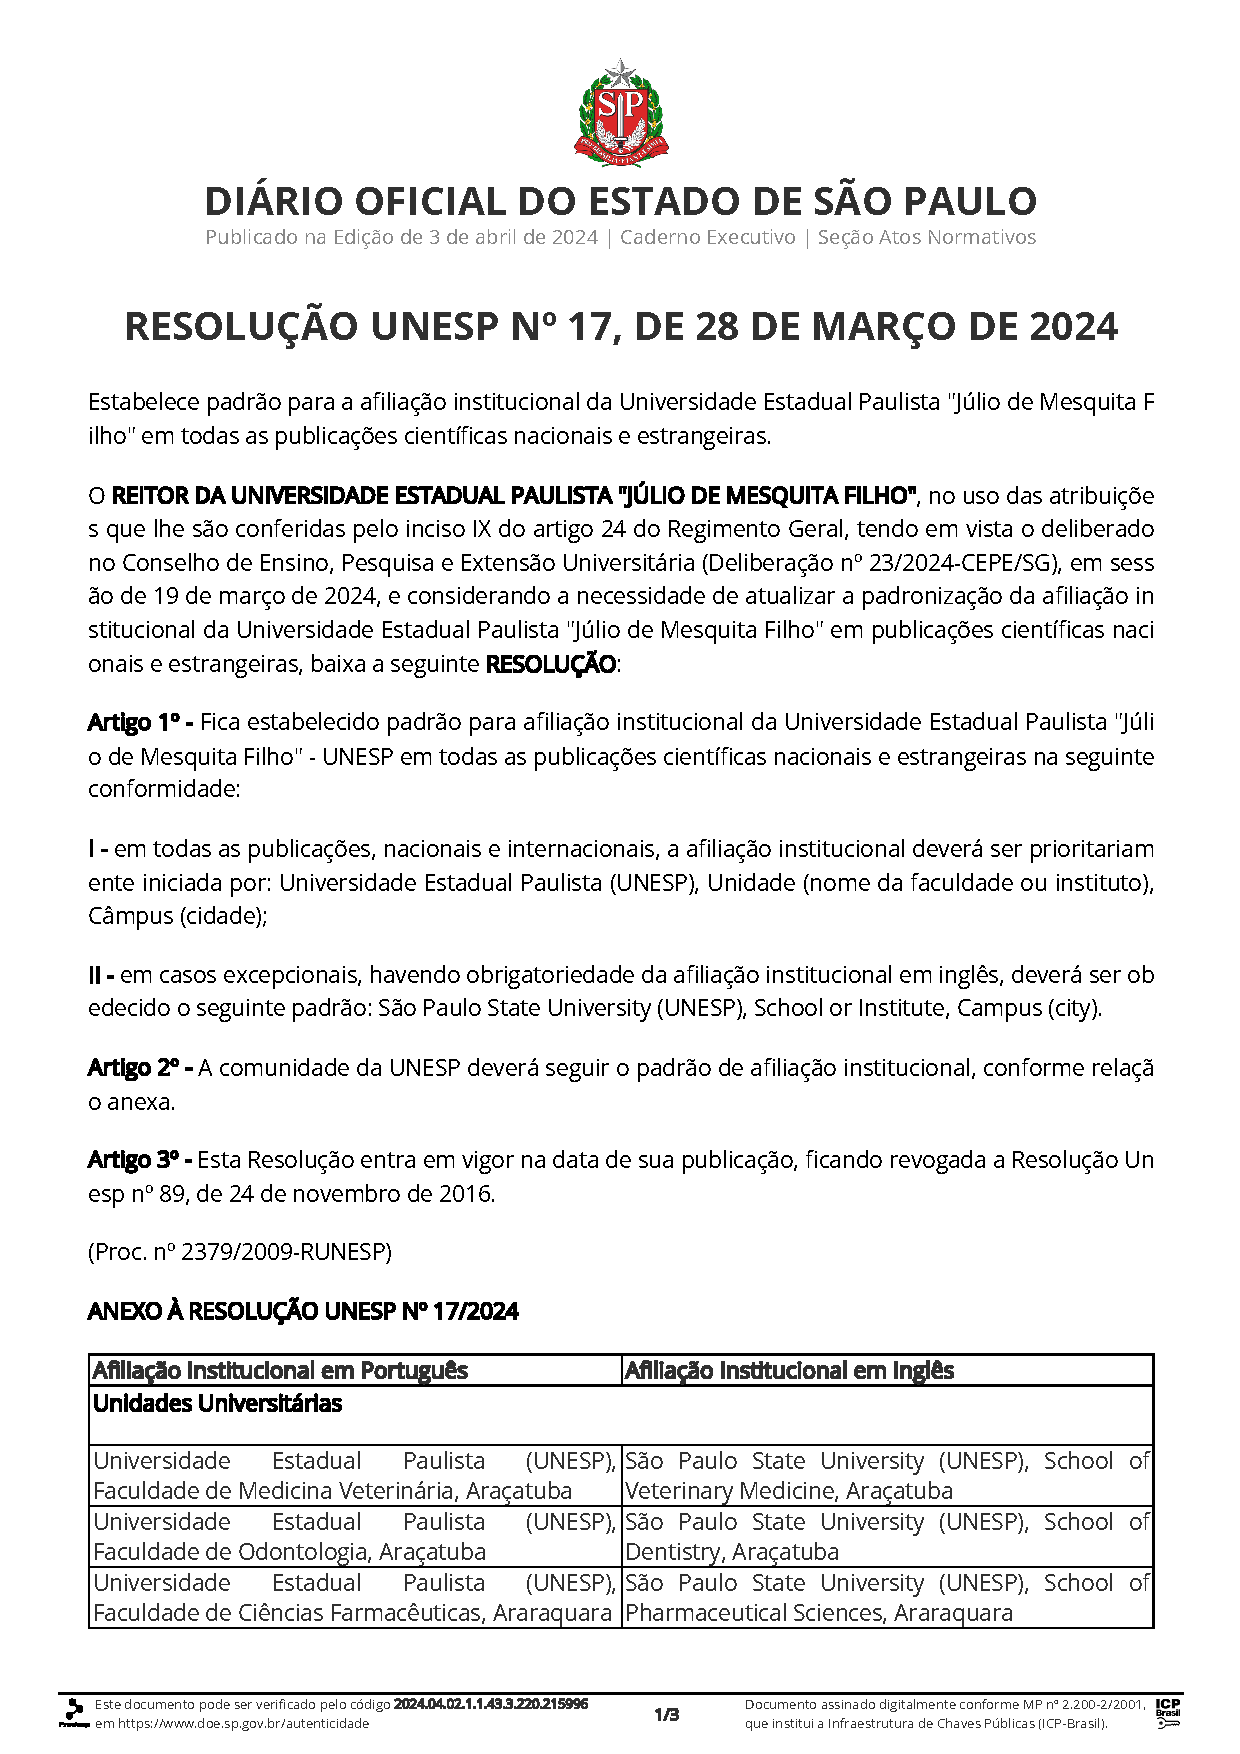
\includepdf[pages=-]{resolucao_unesp17-2024.pdf}

         
    \end{anexosenv}
    \newpage
     %------------------------------------------------------------------------------------%
    % D A D O S   C U R R I C U L A R E S 
    % 
    % OBRIGATÓRIO PARA PÓS-GRADUAÇÃO.
    % Inserir a data inicial e final de cada formação acadêmica. 
     %usar esses comandos para incluir o dados curriculares e que apareça no sumário: \clearpage   %\chapter*{DADOS CURRICULARES} \addcontentsline{toc}{chapter}{DADOS CURRICULARES} 
    %Para os alunos que não precisarem de uma folha de dados curriculares em seu trabalho, basta apagar todo o código dessa seção.
    %------------------------------------------------------------------------------------%
      \clearpage
    \chapter*{DADOS CURRICULARES} \addcontentsline{toc}{chapter}{DADOS CURRICULARES}

    \setlength{\extrarowheight}{5pt}

    \begin{table}[H]
    \centering
      \begin{tabularx}{\textwidth}{|p{3.5cm}|X|}
        \hline
        \rowcolor{black!5}\multicolumn{2}{|p{\columnwidth-15pt}|}{\centering\textbf{IDENTIFICAÇÃO}}\\
        \hline
        
        \multirow{2}{*}{} & \nomeDoAutor\\
        & Data nasc.\\ \hline
        
        \textbf{Nacionalidade} & Nacionalidade do(a) autor(a)\\ \hline
        
        \multirow{2}{*}{\parbox{3.5cm}{\textbf{Nome em citações bibliográficas}}} & Sobrenome, Nome\\
        & Sobrenome, N.\\ \hline
        
        \textbf{Currículo Lattes} & URL\\ \hline
        
        \textbf{ORCID} & URL\\ \hline
        
        \textbf{Outro identificador} & URL\\ \hline
        
        \rowcolor{black!5}\multicolumn{2}{|p{\columnwidth-15pt}|}{\centering\textbf{FORMAÇÃO ACADÊMICA}}\\
        \hline

        \multirow{2}{*}{\parbox{3.5cm}{\textbf{0000/9999}}} & Formação acadêmica (nome do curso e titulação)\\
        & Instituição de ensino\\ \hline

        \multirow{2}{*}{\parbox{3.5cm}{\textbf{0000/9999}}} & Formação acadêmica (nome do curso e titulação)\\
        & Instituição de ensino\\ \hline

        \rowcolor{black!5}\multicolumn{2}{|p{\columnwidth-15pt}|}{\centering\textbf{PRODUÇÃO BIBLIOGRÁFICA}}\\
        \hline

        \multicolumn{2}{|p{\columnwidth-15pt}|}{SOBRENOME, N. .; SOBRENOME, N. Título: subtítulo. \textit{In:} NOME DO EVENTO, 17., 2012, Cidade de realização. \textbf{Anais} […]. Cidade de publicação: Editora, 2012. p. 9-23.}\\
        \hline

        \rowcolor{black!5}\multicolumn{2}{|p{\columnwidth-15pt}|}{\centering\textbf{PARTICIPAÇÃO EM BANCAS E ORIENTAÇÕES}}\\
        \hline

        \multicolumn{2}{|p{\columnwidth-15pt}|}{\centering\textbf{Bancas de trabalhos de conclusão}}\\
        \hline

        \multicolumn{2}{|p{\columnwidth-15pt}|}{SOBRENOME, N.; SOBRENOME, N.; SOBRENOME, N. Participação em banca de Nome Completo do Aluno. \textbf{Título do trabalho}. 2021. Dissertação (Mestrado em Nome do curso) - Nome da Universidade, Cidade, 2021.}\\
        \hline

        \multicolumn{2}{|p{\columnwidth-15pt}|}{\centering\textbf{Orientações}}\\
        \hline

        \multicolumn{2}{|p{\columnwidth-15pt}|}{SOBRENOME, N. \textbf{Título}: subtítulo. 2011.Orientador:  Nome Completo do Orientador. 2011. Trabalho de Conclusão de Curso (Graduação em Nome do Curso) - Nome da Universidade, Cidade, 2011.}\\
        \hline

        \rowcolor{black!5}\multicolumn{2}{|p{\columnwidth-15pt}|}{\centering\textbf{PARTICIPAÇÃO EM EVENTOS CIENTÍFICOS}}\\
        \hline

        \multicolumn{2}{|p{\columnwidth-15pt}|}{NOME DO EVENTO, 17., 2012, (Cidade de realização). Título do trabalho apresentado: subtítulo. 2012. (Seminário).}\\

        \multicolumn{2}{|p{\columnwidth-15pt}|}{NOME DO EVENTO, 7., 2017, (Cidade de realização). Mini-curso: Título do minicurso. 2017. (Seminário).}\\

        
        
        \hline
      \end{tabularx}
    \end{table}
    
    \newpage
                  
    
\end{document}

